\scanpage{3}

\deleted{Soit $A=\coprod_{i\geq0}A_i$ un anneau gradué, à degrés $\geq0$ et soit $\hat A=\prod_{i\geq0}A_i$ le complété pour la filtration canonique. Si cette dernière est \unsure{adique} et $A$ noeth. [p.ex. $A_0$ noeth., $A$ engendré sur $A_{\unsure{0}}$ par $A_1$, $A_1$ de type fini sur $A_0$] alors $\hat A$ est \deleted{\unsure{plat}} plat sur $A$. Pour tout $A$-module $M$, nous posons}
\deleted{\[
\hat M=M\otimes_A\hat A
\]}
\deleted{Supposons que $M$ soit lui-même gradué, et de type fini, alors on a un isom naturel}
\deleted{\[
\hat M=\prod_iM_i.
\]}
\deleted{Si $M$ satisfait seulement TF, alors il existe une suite exacte}
\deleted{\diagram{\begin{tikzcd}[ampersand replacement=\&]
0\arrow[r,dash]\&M''\arrow[r,dash]\&M\arrow[r,dash]\&M'\arrow[r,dash]\&0
\end{tikzcd}}}
\inserted{\deleted{$[M'=$}}
\deleted{$M'$ à degrés majorés, $M''$ de type fini, d'où}
\margin{\inserted{\figure{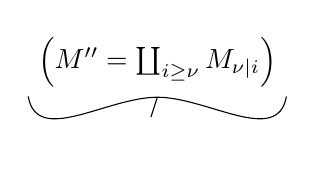
\begin{tikzpicture}
\node(n){$\left(M''=\coprod_{i\geq\nu}M_{\unsure{\nu|i}}\right)$};
\draw(n.south west) to[out=-80,in=180] (0,-.45) to[out=0,in=-100] (n.south east);
\draw(0,-.45)--(-.08,-.7);
\end{tikzpicture}}}}
\deleted{\diagram{\begin{tikzcd}[ampersand replacement=\&]
0\arrow[r,dash]\&\hat M''\arrow[r,dash]\&\hat M\arrow[r,dash]\&\hat M^{\unsure{\prime|\prime\prime}}\arrow[r,dash]\&0
\end{tikzcd}}}
\deleted{Et l'on a}
\deleted{\[
\hat M''=\prod_{i\geq\nu}M_i''=\prod_{i\geq\nu}M_i
\qquad
\hat M'\simeq M'
\]}
\deleted{comme on voit de suite [car $M'$ est \deleted{\unsure{annulé}} loc. annulé par des idéaux de définition].}

\deleted{Donc $\hat M$ est fait des sommes $\sum_{i\in\mathbf Z}x_i$ telles que $x_i\unsure{=|\neq}0$ pour $i\longrightarrow-\infty$.}
\margin{\inserted{\uuline{En tous cas} \unsure{on voit que} $M\mapsto\hat M$ sur les modules \uline{gradués}, \figure{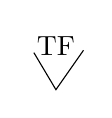
\begin{tikzpicture}\node at(0,.3){\unsure{TF}};\draw(-.28,.22)--(0,-.25)--(.35,.25);\end{tikzpicture}} est exact et \uline{fidèle}}}

\mspage{2}
